\chapter{Stability Simulation}
\label{cap:stabilitysimulation}

This section presents the results of the simulations that have been done to scrutinize the impact of \ac{MV} on the ability to build large \mxpufs.
The first simulation verifies if the introduced principle of \ac{MV} improves the stability of \apuf.
An improvement of the stability of the \apufs is the requirement to create large \xpufs.
In the second simulation the needed number of votes for \ac{MV} in combination with \xpufs, to reach a given stability, is studied.
Finally, the stability distribution of \mxpufs is simulated to compare its results with the stability distribution of an \apuf that is used as reference.

%older: To study the impact of \ac{MV} on the stability of \apufs a simulation approximates the stability of \mpufs and \mxpufs.
% old: To study the impact of \ac{MV} on the stability of \pufs a simulation approximates their stability values.
% younger: Simulations approximate the stability values of \pufs to assess the impact of \ac{MV} on them.
To approximate the stability values of \pufs and to assess the impact of \ac{MV}, simulations with similar configurations are required.
All simulations use a $\sigmaSNoise/\sigmaModel$ ratio of $1/30$ and additional $\sigmaANoise = 0.5$.
Yet since this is a comparison, the ratio does not matter, as explained in Sec.\ \ref{sec:pufsimulation}.

% Nils: maybe code appendix
% Stability distribution of a n = 32 single Arbiter evaluated 100 times! ( 2^16 challenges)
% Backup: 
% \begin{figure}[!ht]
% 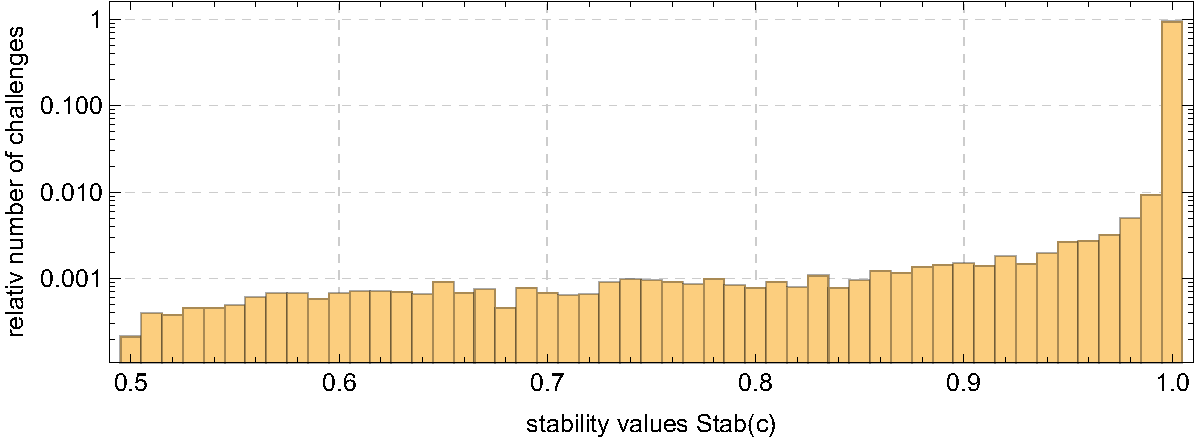
\includegraphics[width=1.00\textwidth]{images/arbiter-stability-distribution-simulation.pdf}
% % \noindent\includegraphics[width=1.00\textwidth, height=3cm, draft]{example-image-a}
% \caption[Challenge stability distribution of an \apuf]{Challenge stability distribution of challenges evaluated by an \apuf using $32$ stages. 
% The graph displays buckets of challenges that are clustered by their stability values.
% Every challenge has been measured $100$ times. The y-axis of the graph shows the number of challenges in relation to all challenges and is scaled logarithmic to figure the wide range of the values.}  % $log_2$
% \label{fig:arbiterstabilitydistribution}
% \end{figure}

\vspace{0.25cm}
\begin{figure}[!ht]
\ifx\coloredfigures\undefined
\todo{Defined variable coloredfigures to be 0 or 1}
\else
	\if\coloredfigures1
	\centering
	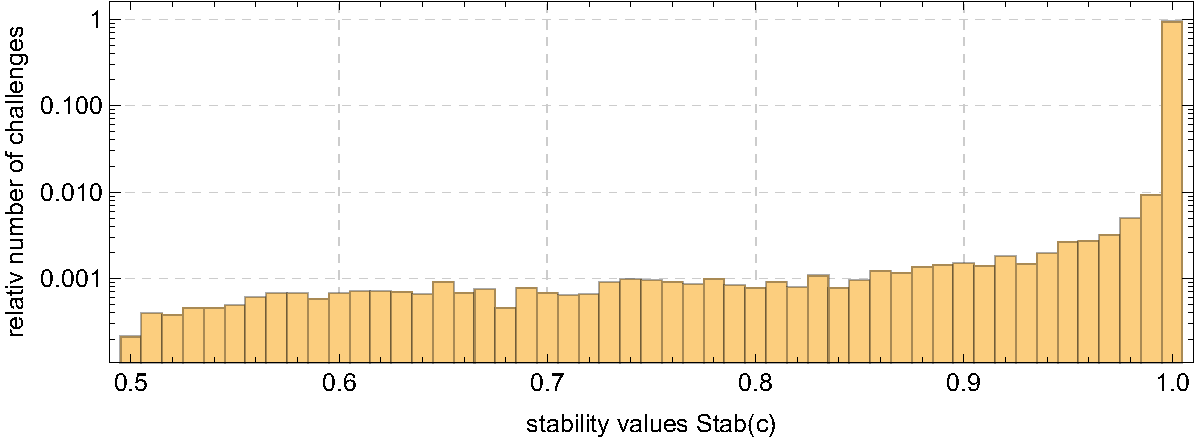
\includegraphics[width=1.00\textwidth]{images/arbiter-stability-distribution-simulation.pdf}
	\else
	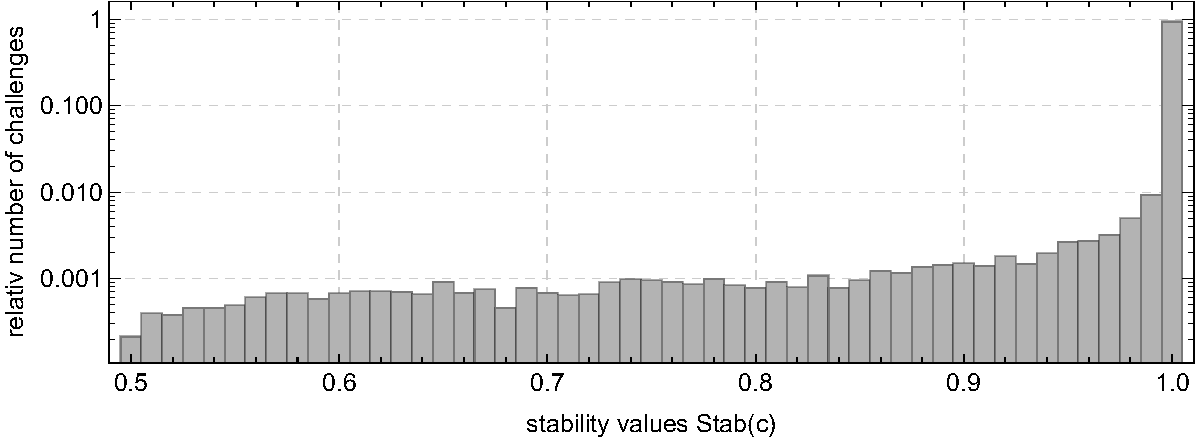
\includegraphics[width=1.00\textwidth]{images/arbiter-stability-distribution-simulation_mono.pdf}
	\fi
\fi
% \noindent\includegraphics[width=1.00\textwidth, height=3cm, draft]{example-image-a}
\caption[Challenge stability distribution of an \apuf]{Challenge stability distribution of challenges evaluated by an \apuf using $32$ stages. 
The graph displays buckets of challenges that are clustered by their stability values.
Every challenge has been measured $100$ times. The y-axis of the graph shows the number of challenges in relation to all challenges and is scaled logarithmic to figure the wide range of the values.}  % $log_2$
\label{fig:arbiterstabilitydistribution}
\end{figure}
\pagebreak

To be able to compare the results of simulations that including \ac{MV}, reference values of \apufs simulations without \ac{MV} are needed.
Consequently, Fig.\ \ref{fig:arbiterstabilitydistribution} shows the stability distribution of an \apuf with $\gls{n} = 32$.
Every challenge has been evaluated $100$ times to approximate its stability.

The very high peak for $\Stab(\gls{c}) = 1$ states that the majority of the challenges already have a very high stability, i.e.\ showed the same result in all $100$ evaluations.
% WRONG: While the other challenges are nearly uniformly distributed with a slightly increase towards the peak i. e. that even the majority of these challenges still has a high stability.
While the number of the other challenges increases for an increase of the stability, i.e.\ the lower the stability the fewer challenges exist.
All challenges with a stability values below a given value are the unstable challenges, as described at the end of Sec.\ \ref{sec:arbiter}.

Since \apufs can have a different number of stages, it could be claimed that this has impact on the stability of the \puf.
% Nils: why is that? -> Paper (lemma 8) (paper not out yet)
Except for very low numbers of $\gls{n}$, Fig.\ \ref{fig:arbiterstabilities} displays that there is no relation and therefore no stability improvement due to the number of used stages. % paper lemma 8
In this simulation for every value of $\gls{n}$ the average of the results of $10$ independent \apufs has been approximated.
A challenge is here considered to be unstable if $\Stab(\gls{c}) < 95\ \%$.

% Percentage of unstable challenges (Stab(c) < 0.95 %) of a random chosen set of challenges of Arbiters of different size n, avg over 10 independent instances ( 2^11 challenges)
% Backup: 
% \begin{figure}[ht]
% 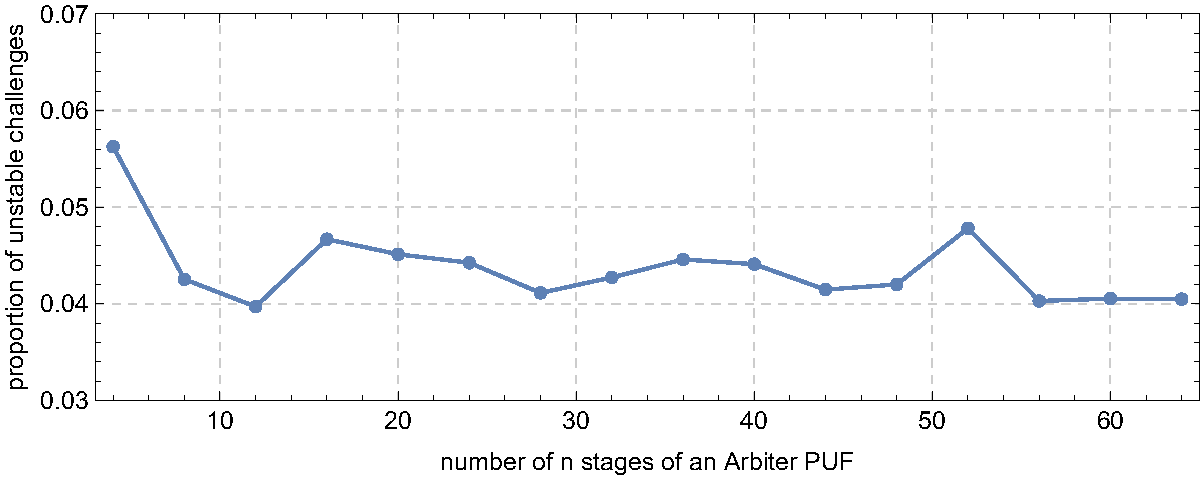
\includegraphics[width=1.00\textwidth]{images/stages-stab-simulation.pdf}
% % \noindent\includegraphics[width=1.00\textwidth, height=3cm, draft]{example-image-a}
% \caption[Proportion of unstable challenges of an \apuf]{Proportion of unstable challenges of a random chosen set of challenges for \apufs with $\gls{n}$ stages. 
% A challenge is unstable when $\Stab(\gls{c}) < 95\ \%$. 
% The results are the average values over $10$ individual \puf instances with the same challenge set.} 
% \label{fig:arbiterstabilities}
% \end{figure}

\vspace{0.25cm}
\begin{figure}[ht]
\ifx\coloredfigures\undefined
\todo{Defined variable coloredfigures to be 0 or 1}
\else
	\if\coloredfigures1
\centering
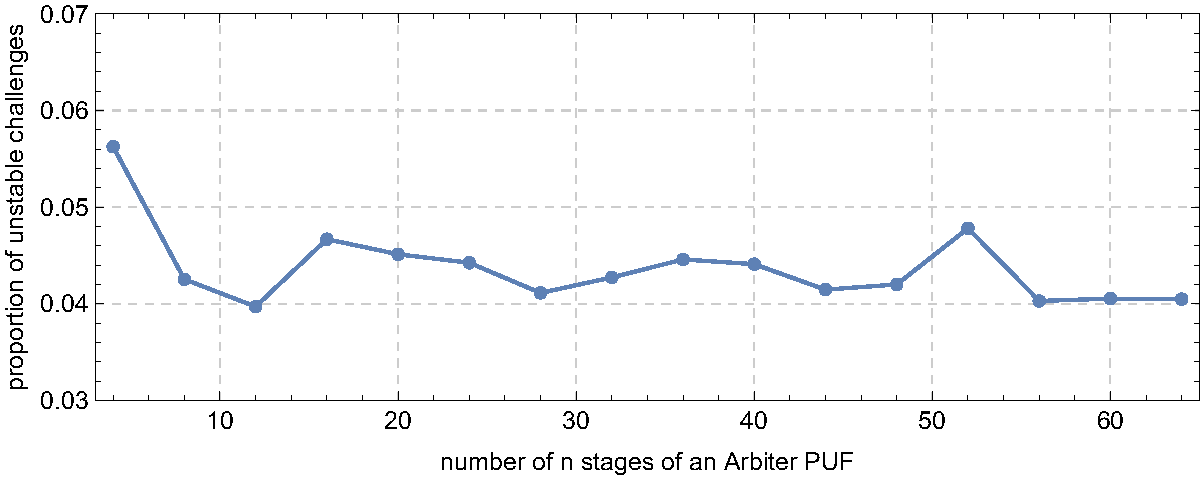
\includegraphics[width=1.00\textwidth]{images/stages-stab-simulation.pdf}
	\else
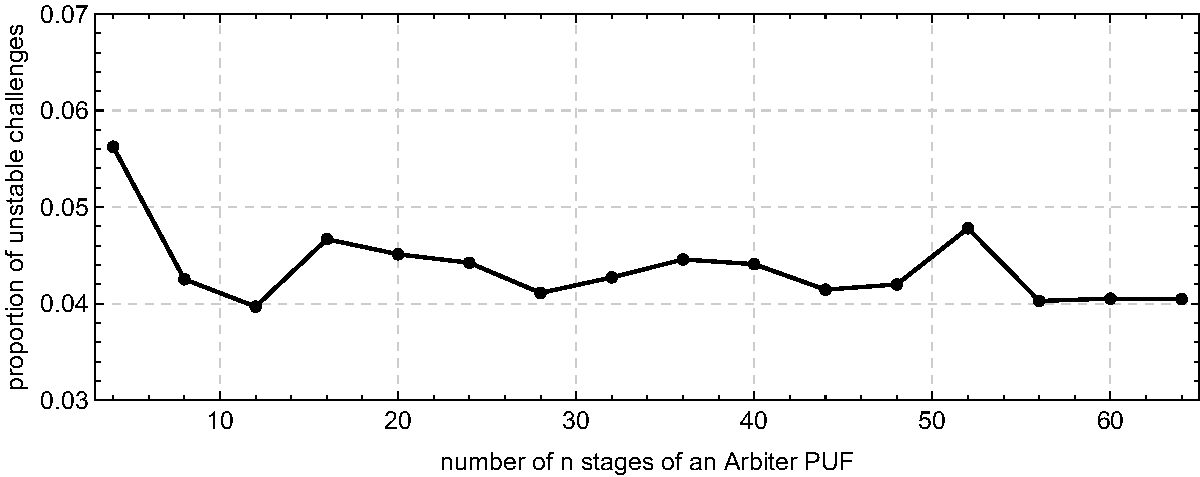
\includegraphics[width=1.00\textwidth]{images/stages-stab-simulation_mono.pdf}
    \fi
\fi
% \noindent\includegraphics[width=1.00\textwidth, height=3cm, draft]{example-image-a}
\caption[Proportion of unstable challenges of an \apuf]{Proportion of unstable challenges of a random chosen set of challenges for \apufs with $\gls{n}$ stages. 
A challenge is unstable when $\Stab(\gls{c}) < 95\ \%$. 
The results are the average values over $10$ individual \puf instances with the same challenge set.} 
\label{fig:arbiterstabilities}
\end{figure}


% simulation values: noise  to model ratio: ref to simulation design!
%========================================

\section{Stability Improvement by Majority Vote}
\label{sec:stabilityimprovementbymajorityvote}

To prove the stability increase achieved by \ac{MV}, Fig.\ \ref{fig:majorityvotestabilityimprovement} shows the decrease of unstable challenges for a growing number of votes.
The \mpuf has size $\gls{n} = 32$ and used challenges are randomly chosen.
Challenges are again considered to be unstable when $\Stab(\gls{c}) < 95\ \%$.
% Old and wrong: Beside the expression of declining unstable challenges the graph has a raising gradient, which means that the improving impact of \ac{MV} subsides with growing $\gls{m}$, as Fig.\ \ref{fig:majorityvotestabilityimprovement} displays.

% Percentage of unstable challenges (Stab(c) < 0.95 %) of a random chosen set of challenges of Arbiters of n=32 for different majority votes (2^11 challenges)
% Backup: 
% \begin{figure}[ht]
% 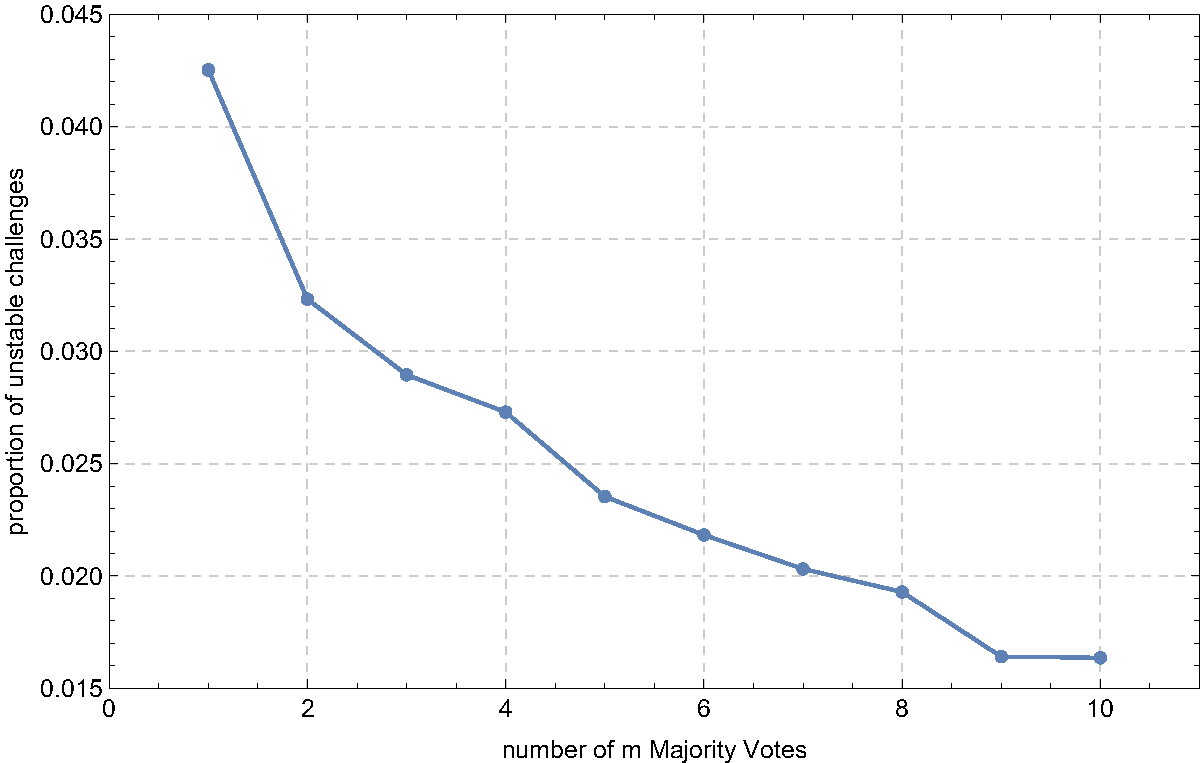
\includegraphics[width=1.00\textwidth]{images/single-votes-stab-simulation.pdf}
% % \noindent\includegraphics[width=1.00\textwidth, height=3cm, draft]{example-image-a}
% \caption[Decrease of unstable challenges of a \mpuf]{The line graph displays the decrease of the proportion of unstable challenges, which have $\Stab(\gls{c}) < 95\ \%$, of a random chosen set of challenges for different number of $\gls{m}$ \acp{MV} of a \mpuf.
% The \mpuf has size $\gls{n} = 32$.
% } %  and clarified by the logarithmic Fig.\ \ref{fig:majorityvotestabilityimprovementloglog}.
% \label{fig:majorityvotestabilityimprovement}
% \end{figure}

\vspace{0.25cm}
\begin{figure}[ht]
\ifx\coloredfigures\undefined
\todo{Defined variable coloredfigures to be 0 or 1}
\else
	\if\coloredfigures1
\centering
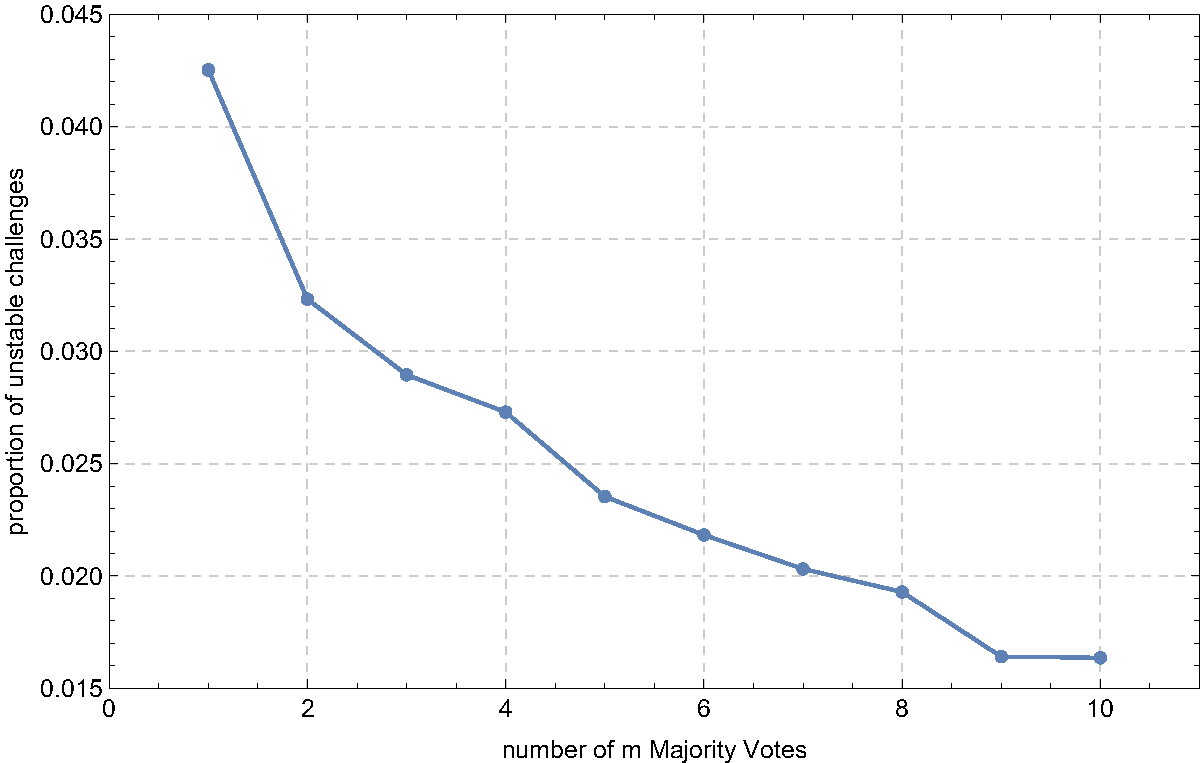
\includegraphics[width=1.00\textwidth]{images/single-votes-stab-simulation.pdf}
	\else
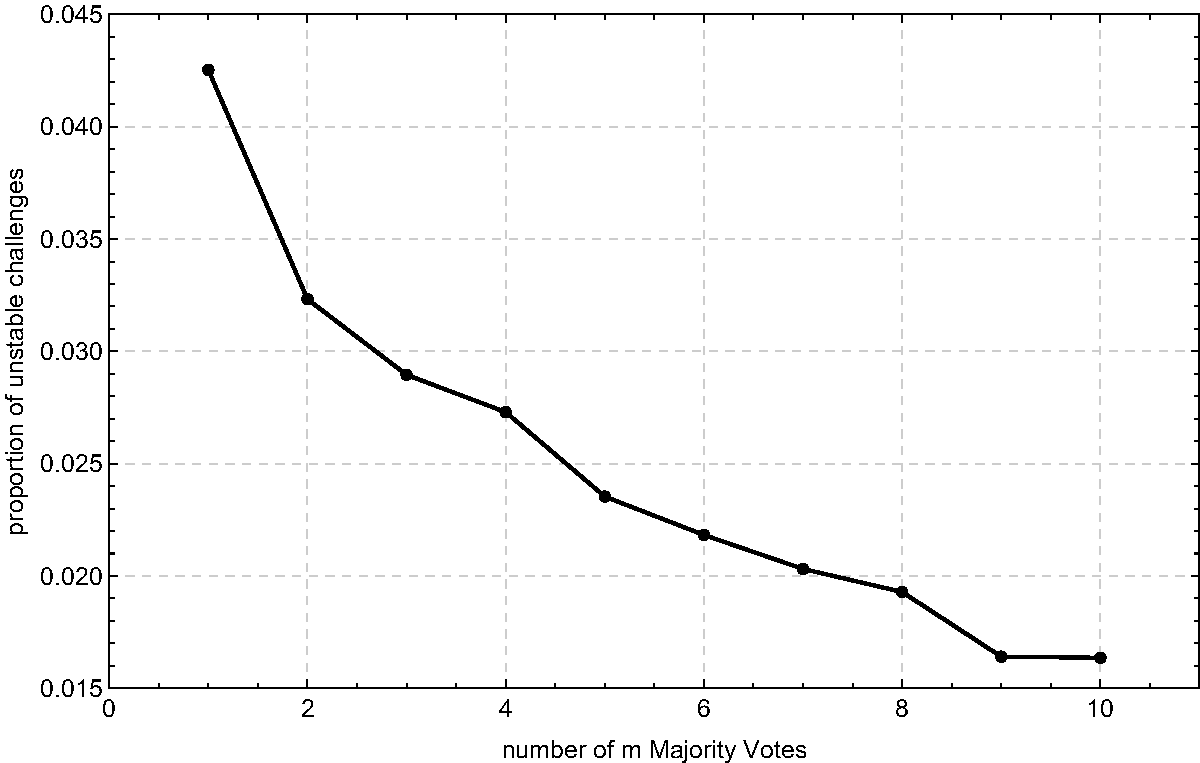
\includegraphics[width=1.00\textwidth]{images/single-votes-stab-simulation_mono.pdf}
    \fi
\fi
% \noindent\includegraphics[width=1.00\textwidth, height=3cm, draft]{example-image-a}
\caption[Decrease of unstable challenges of a \mpuf]{The line graph displays the decrease of the proportion of unstable challenges, which have $\Stab(\gls{c}) < 95\ \%$, of a random chosen set of challenges for different number of $\gls{m}$ \acp{MV} of a \mpuf.
The \mpuf has size $\gls{n} = 32$.
} %  and clarified by the logarithmic Fig.\ \ref{fig:majorityvotestabilityimprovementloglog}.
\label{fig:majorityvotestabilityimprovement}
\end{figure}

Beside the expression of declining unstable challenges the graph has a raising gradient, as Fig.\ \ref{fig:majorityvotestabilityimprovement} displays.
This could lead to the assumption that the improving impact of \ac{MV} subsides with growing $\gls{m}$.
To clarify this the logarithmic Fig.\ \ref{fig:majorityvotestabilityimprovementloglog} has been created with the same values.
It displays a nearly linear graph that suggest that there is no mitigation of the stability improving impact of \ac{MV} with increasing $\gls{m}$.
% Old: Hence the relative stability improvement is highest with the first increase of $\gls{m}$ as the beginning of the graph shows.
Nevertheless, the relative stability improvement is highest with the first increase of $\gls{m}$, as the beginning of the graph in Fig.\  \ref{fig:majorityvotestabilityimprovement} shows.

% Backup: 
% \begin{figure}[htp]
% 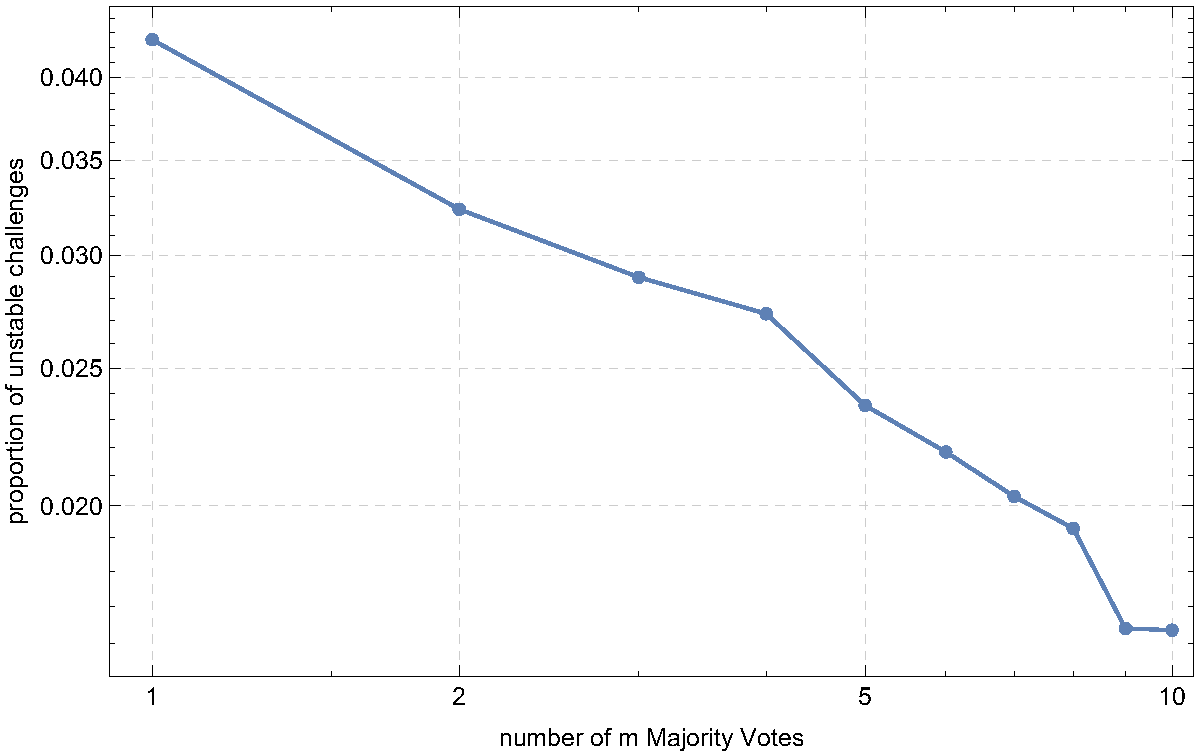
\includegraphics[width=1.00\textwidth]{images/single-votes-stab-simulation_loglog.pdf}
% % \noindent\includegraphics[width=1.00\textwidth, height=3cm, draft]{example-image-a}
% \caption[Decrease of unstable challenges of a \mpuf logarithmic]{The line graph shows the decrease of the proportion of unstable challenges similar to Fig.\ \ref{fig:majorityvotestabilityimprovement}, yet in logarithmic scale. The  linear course of the graph suggests that there is no mitigation in the stability improving impact of \ac{MV} with growing $\gls{m}$ used for \mpufs.} 
% \label{fig:majorityvotestabilityimprovementloglog}
% \end{figure}

\begin{figure}[htp] % htp
\ifx\coloredfigures\undefined
\todo{Defined variable coloredfigures to be 0 or 1}
\else
	\if\coloredfigures1
\centering
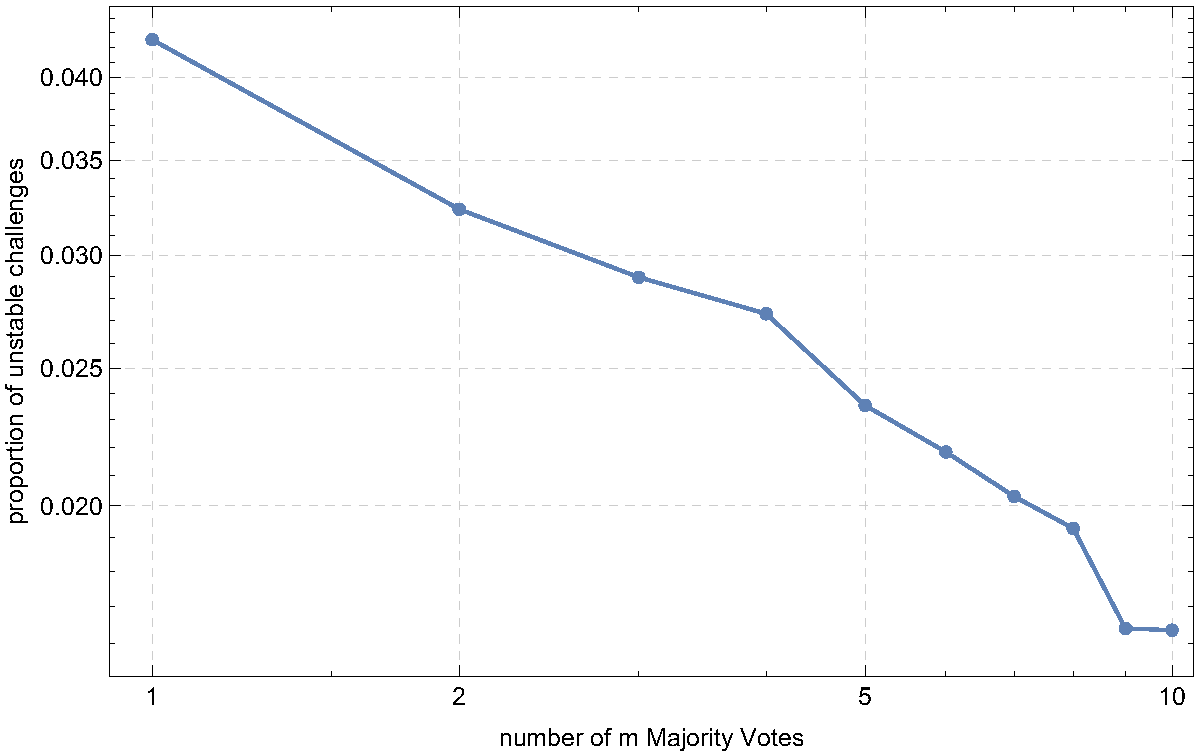
\includegraphics[width=1.00\textwidth]{images/single-votes-stab-simulation_loglog.pdf}
	\else
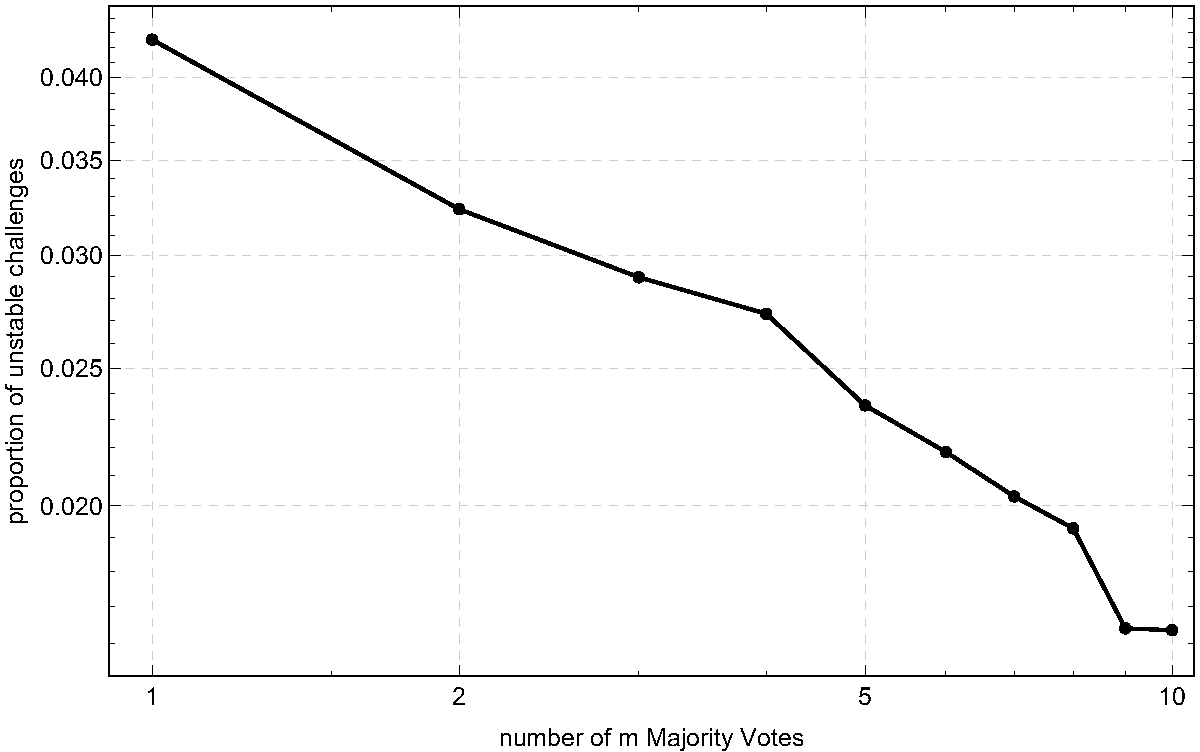
\includegraphics[width=1.00\textwidth]{images/single-votes-stab-simulation_loglog_mono.pdf}
    \fi
\fi
% \noindent\includegraphics[width=1.00\textwidth, height=3cm, draft]{example-image-a}
\caption[Decrease of unstable challenges of a \mpuf logarithmic]{The line graph shows the decrease of the proportion of unstable challenges similar to Fig.\ \ref{fig:majorityvotestabilityimprovement}, yet in logarithmic scale. The  linear course of the graph suggests that there is no mitigation in the stability improving impact of \ac{MV} with growing $\gls{m}$ used for \mpufs.} 
\label{fig:majorityvotestabilityimprovementloglog}
\end{figure}

\begin{figure}[!htp] %!htp
\ifx\coloredfigures\undefined
\todo{Defined variable coloredfigures to be 0 or 1}
\else
	\if\coloredfigures1
\centering
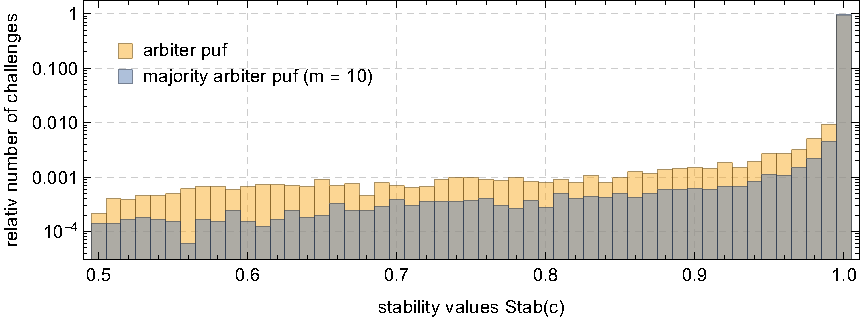
\includegraphics[width=1.00\textwidth]{images/comparison-arbiter-stability-distribution-majority-arbiter-stability-distribution.pdf}
	\else
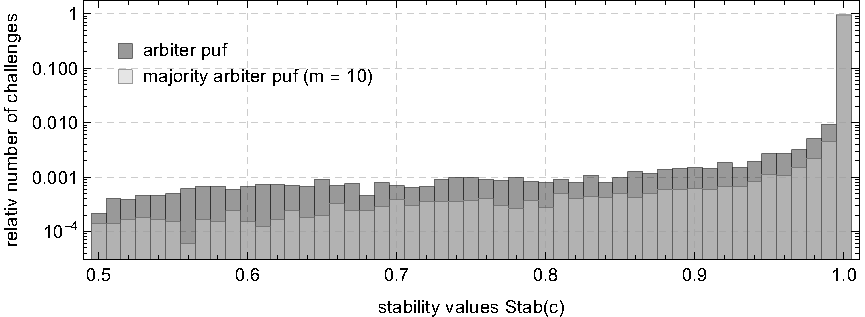
\includegraphics[width=1.00\textwidth]{images/comparison-arbiter-stability-distribution-majority-arbiter-stability-distribution_mono.pdf}
    \fi
\fi
% \noindent\includegraphics[width=1.00\textwidth, height=3cm, draft]{example-image-a}
\caption[Challenge stability distribution of a \mpuf]{Challenge stability distribution of challenges evaluated by a \mpuf using $32$ stages and $\gls{m} = 10$ in comparison to the distribution of an \apuf, as shown in Fig.\ \ref{fig:arbiterstabilitydistribution}. Challenges that have been measured $100$ times each are clustered by their stability. The y-axis displays the number of challenges relative to all challenges and is scaled logarithmic to figure the wide range of the values.} 
\label{fig:comparisonarbiterstabilitydistributionmajorityarbiterstabilitydistribution}
\end{figure}

The Fig.\ \ref{fig:majorityvotestabilityimprovement} and Fig.\ \ref{fig:majorityvotestabilityimprovementloglog} show that \ac{MV} improves the stability of an \apuf remarkable. 
For more details on the challenge stability distribution Fig.\ \ref{fig:comparisonarbiterstabilitydistributionmajorityarbiterstabilitydistribution} shows the challenge stability distribution of a \mpuf with $\gls{m} = 10$ \acp{MV} in comparison to the challenge stability distribution of an \apuf, as shown in the beginning of this chapter.
In the comparison of the figures the reduced number of challenges with lowered stability can be seen.
This stability increase of \mpufs can be used to build large \mxpufs, which are examined in Sec.\ \ref{sec:majorityvotegrowth}.

% Old: only the stability values, no comparison
% \begin{figure}[ht]
% 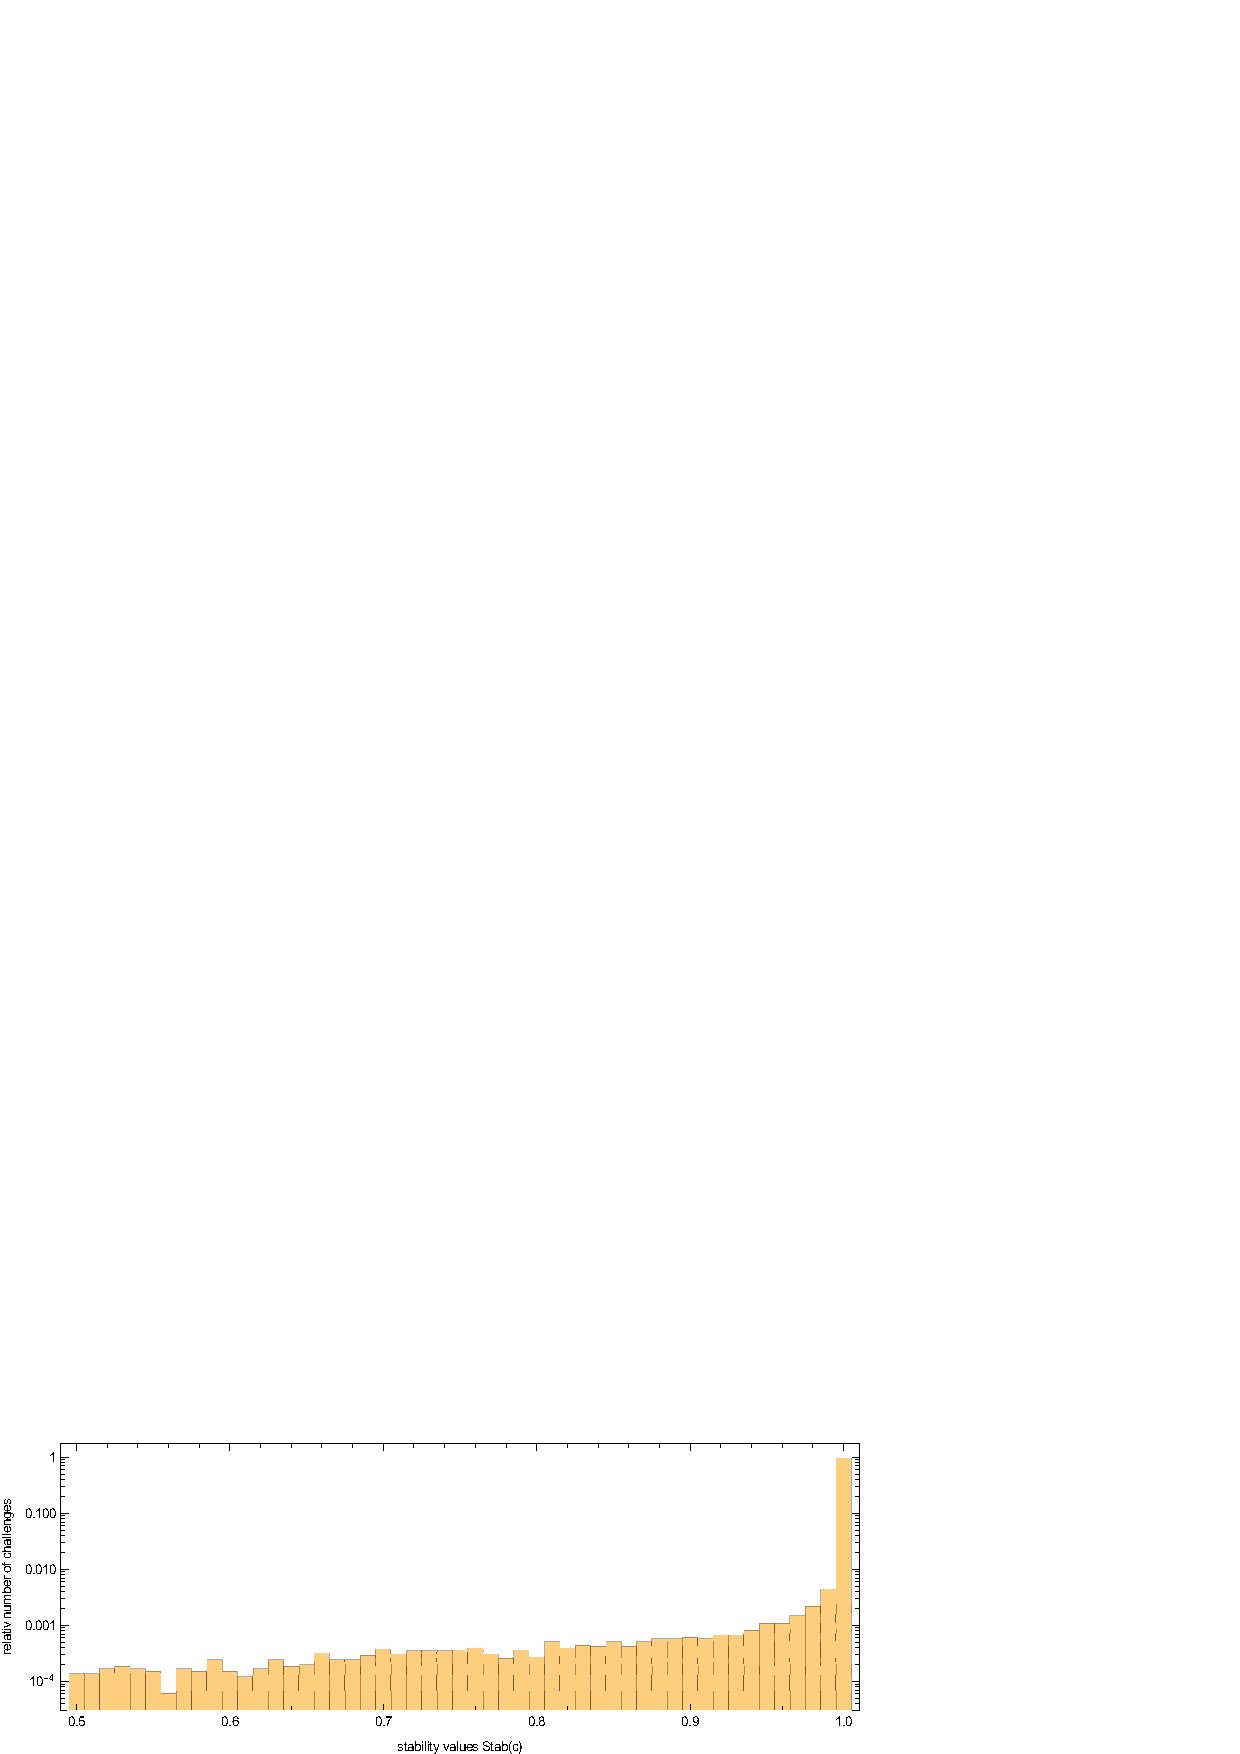
\includegraphics[width=1.00\textwidth]{images/majority-arbiter-stability-distribution-simulation.pdf}
% % \noindent\includegraphics[width=1.00\textwidth, height=3cm, draft]{example-image-a}
% \caption[Challenge stability distribution of a \mpuf]{Challenge stability distribution of challenges evaluated by a \mpuf using $32$ stages and $\gls{m} = 10$. Challenges that have been measured $100$ times each are clustered by their stability. The y-axis displays the number of challenges relative to all challenges and is scaled logarithmic to figure the wide range of the values.} 
% \label{fig:majorityarbiterstabilitydistribution}
% \end{figure}

% Backup: 
% \begin{figure}[!htp]
% 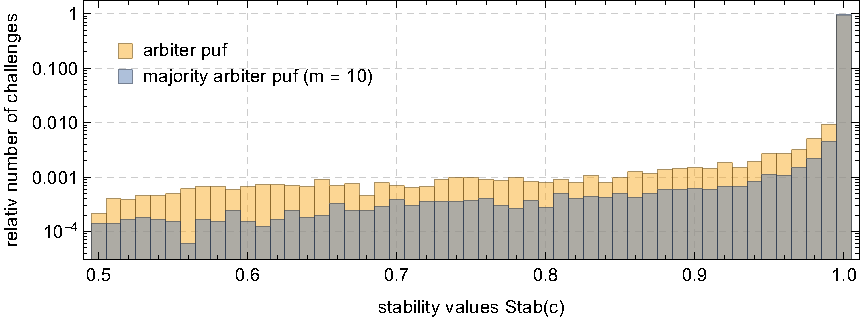
\includegraphics[width=1.00\textwidth]{images/comparison-arbiter-stability-distribution-majority-arbiter-stability-distribution.pdf}
% % \noindent\includegraphics[width=1.00\textwidth, height=3cm, draft]{example-image-a}
% \caption[Challenge stability distribution of a \mpuf]{Challenge stability distribution of challenges evaluated by a \mpuf using $32$ stages and $\gls{m} = 10$ in comparison to the distribution of an \apuf, as shown in Fig.\ \ref{fig:arbiterstabilitydistribution}. Challenges that have been measured $100$ times each are clustered by their stability. The y-axis displays the number of challenges relative to all challenges and is scaled logarithmic to figure the wide range of the values.} 
% \label{fig:comparisonarbiterstabilitydistributionmajorityarbiterstabilitydistribution}
% \end{figure}


%========================================

\section{Majority Vote Increase for Majority \acs{XOR} \apufs}
\label{sec:majorityvotegrowth}
% Number of needed votes for k large xor arbiter to achieve a certain stability

As only \xpufs that are large in $\gls{k}$ can not be modeled successfully by known attacks, it is the purpose to be able to create large \xpufs, which have to be stable to produce a reliable output. % arbitrary
To achieve this through \ac{MV}, the number of $\gls{m}$ votes has to be increased with a growth in $\gls{k}$, as shown in Sec.\ \ref{sec:majorityxorarbiter}.

Yet the growth rate of $\gls{m}$ must not be too high otherwise the time to evaluate a challenge would grow too large with large \xpufs as well. %, like exponential, 
% Old: To show that this high stability can be reached using a polynomial number of $\gls{m}$ \acp{MV} $\gls{k}$ parallel \mpufs for different values of $\gls{k}$ are simulated.
To show that this high stability can be reached using a polynomial number of $\gls{m}$ \acp{MV}, multiple \mxpufs are simulated.
These \mxpufs consists of different numbers of $k$ parallel \mpufs.
% Oldold: The simulation measures the stability values of every challenge by multiple evaluations and finds the necessary number of \ac{MV} by binary search.
% Old:
% The simulation measures the stability values of every challenge evaluated by the \mxpuf through multiple evaluations
% It then approximates the number of $m$ \acp{MV} to reach $\Pr[\protect\Stab(\gls{c}) \ge 95\ \%] \ge 95\ \%$ for different numbers of $k$ by binary search.

% Backup: 
% \begin{figure}[ht]
% 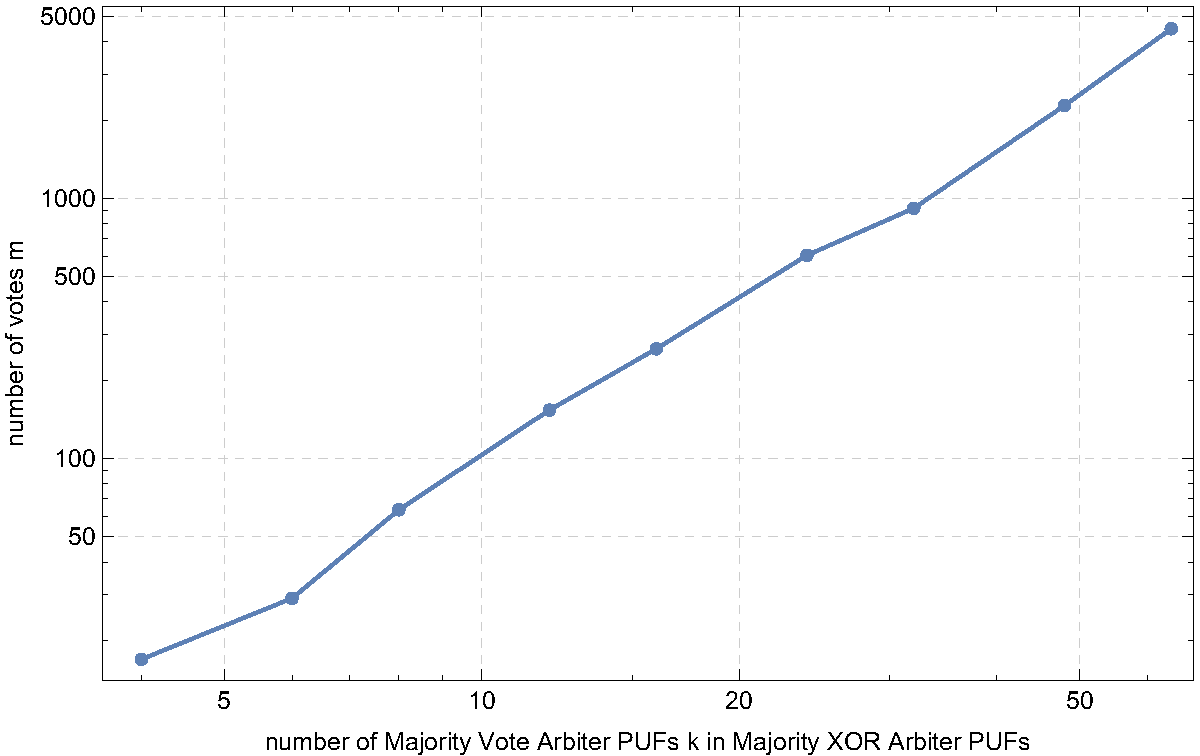
\includegraphics[width=1.00\textwidth]{images/votes-stab-simulation.pdf}
% % \noindent\includegraphics[width=1.00\textwidth, height=3cm, draft]{example-image-a}
% \caption[Number of votes needed for large Majority \acs{XOR} \apufs]{Minimum number of votes needed to reach $\Pr[\protect\Stab(\gls{c}) \ge 95\ \%] \ge 95\ \%$ for a uniformly random chosen challenge $\gls{c}$ for different numbers of $\gls{k}$ \apufs. 
% The simulations uses $\gls{n} = 16$, but the results are independent of $\gls{n}$, as shown in Fig.\ \ref{fig:arbiterstabilities}. 
% The linear graph shown in a log-log-graph confirms the polynomial growing number $\gls{m}$ of \acp{MV} of the degree $1$.
% The results are the average values over $10$ individual \puf instances with independent challenge sets.} 
% \label{fig:majorityvotegrowth}
% \end{figure}

\begin{figure}[!ht]
\ifx\coloredfigures\undefined
\todo{Defined variable coloredfigures to be 0 or 1}
\else
	\if\coloredfigures1
\centering
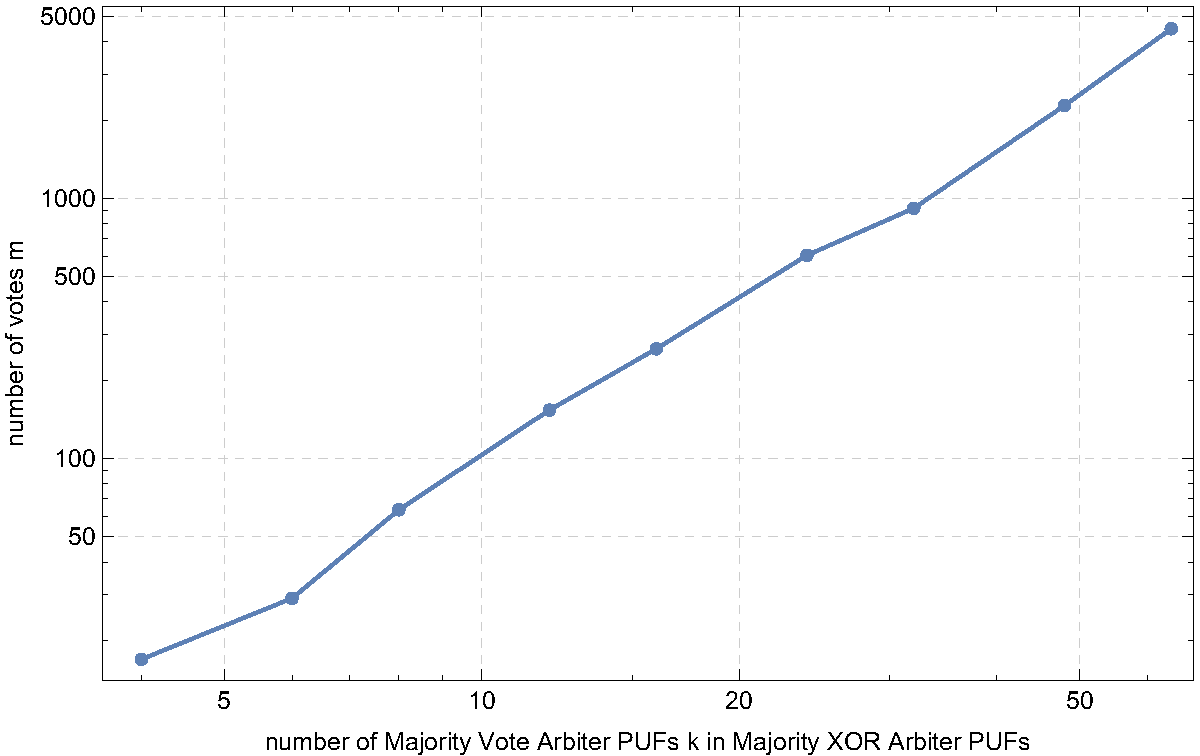
\includegraphics[width=1.00\textwidth]{images/votes-stab-simulation.pdf}
	\else
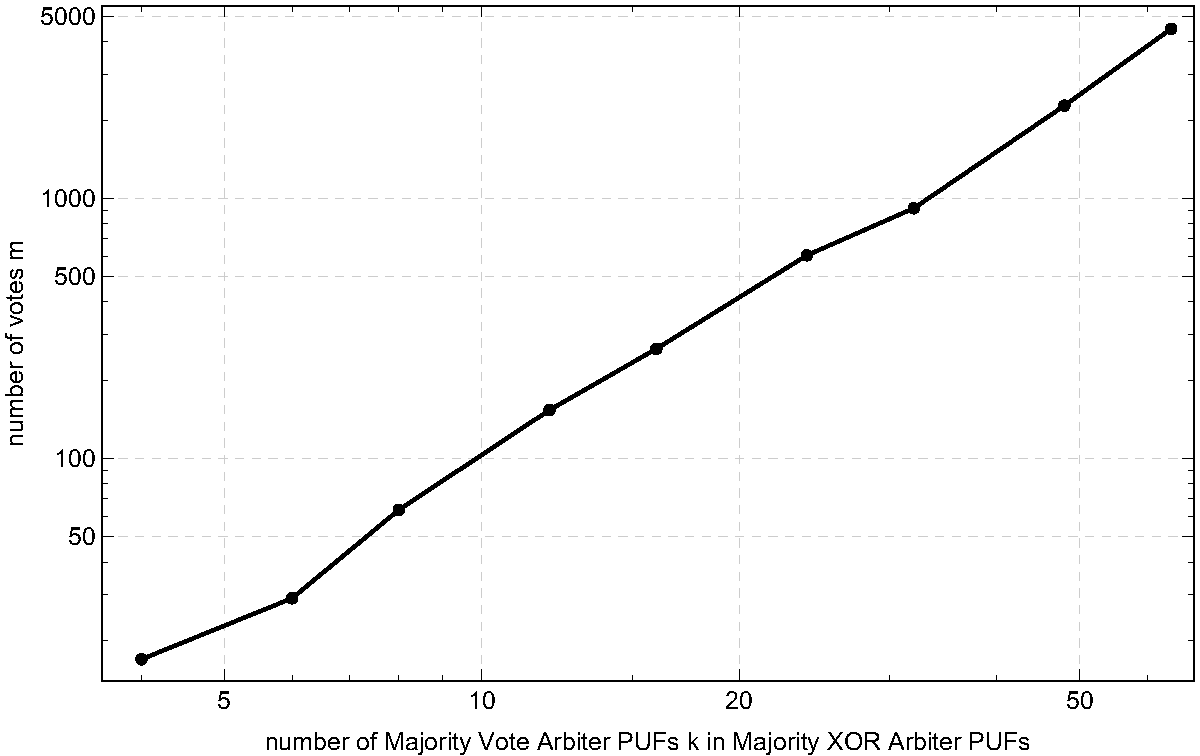
\includegraphics[width=1.00\textwidth]{images/votes-stab-simulation_mono.pdf} 
    \fi
\fi
% \noindent\includegraphics[width=1.00\textwidth, height=3cm, draft]{example-image-a}
\caption[Number of votes needed for large Majority \acs{XOR} \apufs]{Minimum number of votes needed to reach $\Pr[\protect\Stab(\gls{c}) \ge 95\ \%] \ge 95\ \%$ for uniformly and randomly chosen challenges $\gls{c}$ for different numbers of $\gls{k}$ \apufs. 
The simulations use $\gls{n} = 16$, but the results are independent of $\gls{n}$, as shown in Fig.\ \ref{fig:arbiterstabilities}. 
The linear graph shown in a log-log-graph confirms the polynomial growing number $\gls{m}$ of \acp{MV} of the degree $1$.
All results are the average values over $10$ individual \puf instances with independent challenge sets.} 
\label{fig:majorityvotegrowth}
\end{figure}

The simulation approximates the number of $m$ \acp{MV} to reach $\Pr[\protect\Stab(\gls{c}) \ge 95\ \%] \ge 95\ \%$ for different numbers of $k$ by binary search.
Therefore, it measures the stability values of every challenge evaluated by the underlying \mpufs through multiple evaluations, calculates the stability values for the \mxpuf, and changes the number of $m$ votes till the stability is reached.

Fig.\ \ref{fig:majorityvotegrowth} shows how many votes are needed to reach a likelihood of $95\ \%$ that uniformly and randomly chosen challenges have a stability of at least $95\ \%$, for different values of $\gls{k}$.
These are upper bounds, as the \ac{XOR} operation increases the stability of a \xpuf marginal, because any even number of incorrect \apuf responses will still yield the desired output of the \xpuf. 
This behavior is not included in the simulation, since the stability values of the challenges are approximated for all \apufs independently.

The polynomial increasing number of votes needed to fulfill the stability requirements for a useful PUF implementation displayed in the Fig.\ \ref{fig:majorityvotegrowth} proves that \xpufs can be built arbitrary large using \ac{MV}.

%========================================
% Figure fig:majorityvotegrowth: maybe add n=8 and n=12, so the reader can see that the results indeed do not change

\section{Stability Distribution of Large Majority \acs{XOR} \apufs}
\label{sec:distributionoflargemxpufs}
% Stability distribution of xor arbiter

To get a more precise exposition of the stability distribution of \mxpufs with large size $\gls{k}$, the stability value for every challenge of a subset of all challenges is simulated.
The results are then compared with the stability distribution of the \apuf.

Only a subset of challenges is used due to the needed simulation computation time.
Nevertheless, this random chosen subset represents the distribution of all challenges. 
All challenge of the subset are evaluated $100$ times to compute their stability values.
The example uses $32$ \mpufs with $32$ stages each.
The number of \acp{MV} needed to reach a stability of $95\ \%$ with a likelihood of $95\ \%$ is chosen from the results of Sec.\ \ref{sec:majorityvotegrowth}.

The challenge stability distribution of a \mxpuf, shown in Fig.\ \ref{fig:comparisonarbiterstabilitydistributionmajorityxorstabilitydistribution}, was achieved by using $\gls{m} = 600$ votes and is roughly equivalent to the distribution of an \apuf displayed in the Fig.\ \ref{fig:arbiterstabilitydistribution} and here for comparison.

% \begin{figure}[ht]
% 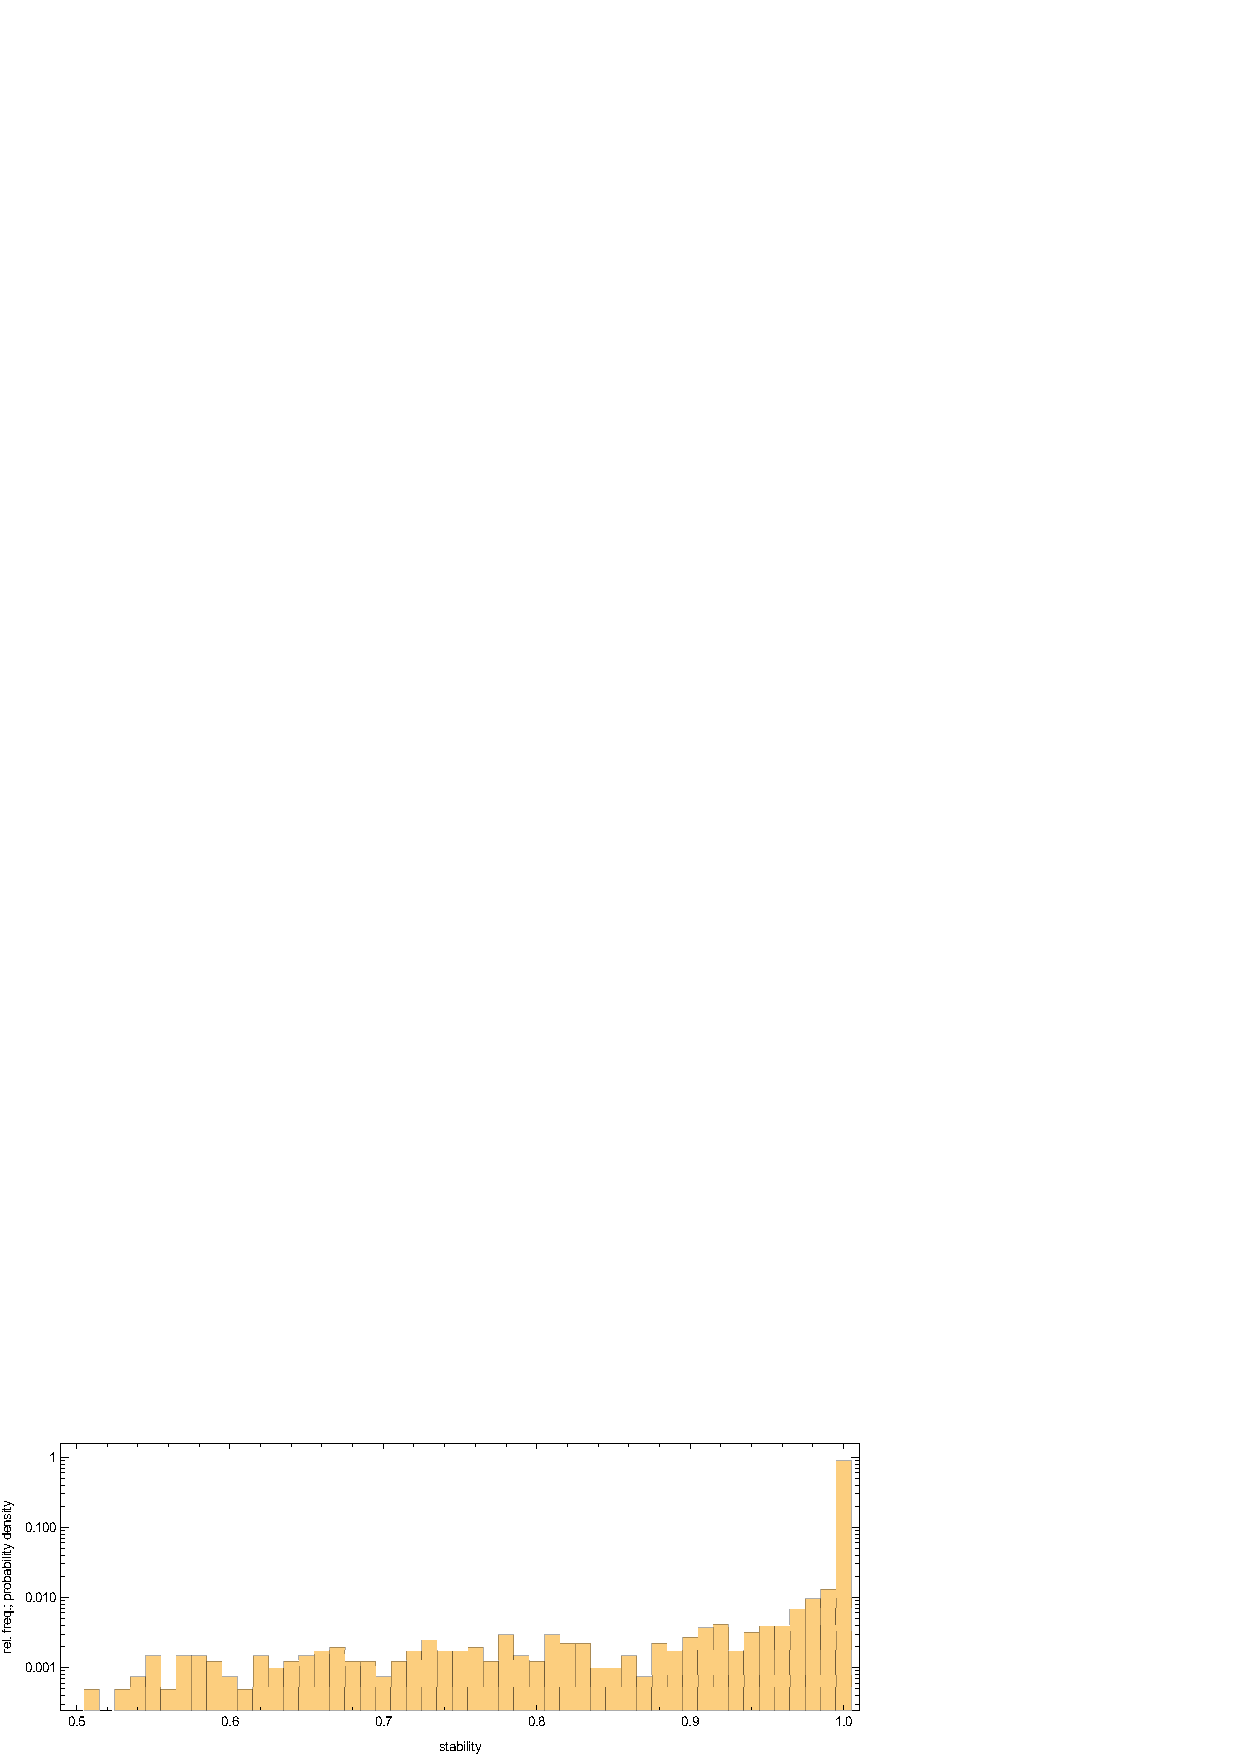
\includegraphics[width=1.00\textwidth]{images/majority-xor-stability-distribution-simulation.pdf}
% % \noindent\includegraphics[width=1.00\textwidth, height=3cm, draft]{example-image-a}
% \caption[Challenge stability distribution of a \mxpuf]{The histogram shows the relative frequency of the challenge stability values clustered into buckets of a \mxpuf with size $\gls{k} = 32$ and $32$ stages each. \ac{MV} uses $\gls{m} = 600$ to reach a stability of $95\ \%$ with likelihood $95\ \%$ for randomly chosen challenges. The distribution and the amount of unstable challenges resembles the stability distribution of a \apuf as displayed in Fig.\ \ref{fig:arbiterstabilitydistribution}.} 
% \label{fig:stabilitydistributionmajorityvote}
% \end{figure}

% Backup:  
% \begin{figure}[ht]
% 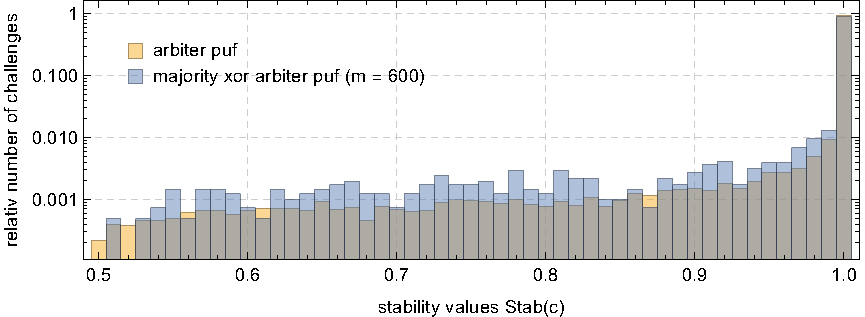
\includegraphics[width=1.00\textwidth]{images/comparison-arbiter-stability-distribution-majority-xor-stability-distribution.pdf}
% % \noindent\includegraphics[width=1.00\textwidth, height=3cm, draft]{example-image-a}
% \caption[Challenge stability distribution of a Majority \acs{XOR} \apuf]{The histogram shows the relative frequency of the challenge stability values clustered into buckets of a \mxpuf with size $\gls{k} = 32$ and $32$ stages each in comparison to the challenge stability distribution of an \apuf, as shown in Fig.\ \ref{fig:arbiterstabilitydistribution}. \ac{MV} uses $\gls{m} = 600$ to reach a stability of $95\ \%$ with likelihood $95\ \%$ for randomly chosen challenges. The distribution and the amount of unstable challenges of the \mxpuf resembles the distribution of a \apuf.} 
% \label{fig:comparisonarbiterstabilitydistributionmajorityxorstabilitydistribution}
% \end{figure}

\vspace{0.25cm}
\begin{figure}[ht]
\ifx\coloredfigures\undefined
\todo{Defined variable coloredfigures to be 0 or 1}
\else
	\if\coloredfigures1
\centering
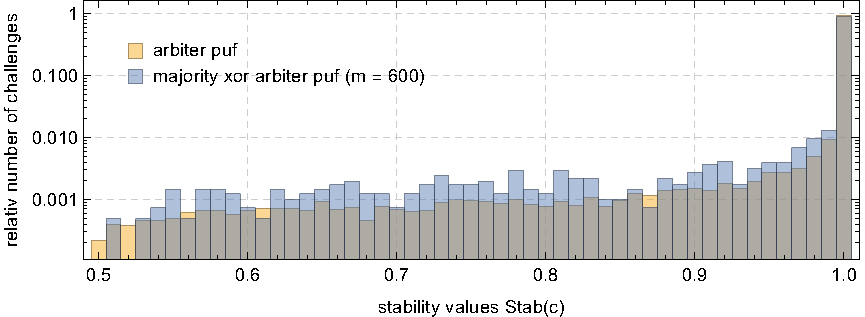
\includegraphics[width=1.00\textwidth]{images/comparison-arbiter-stability-distribution-majority-xor-stability-distribution.pdf}
	\else
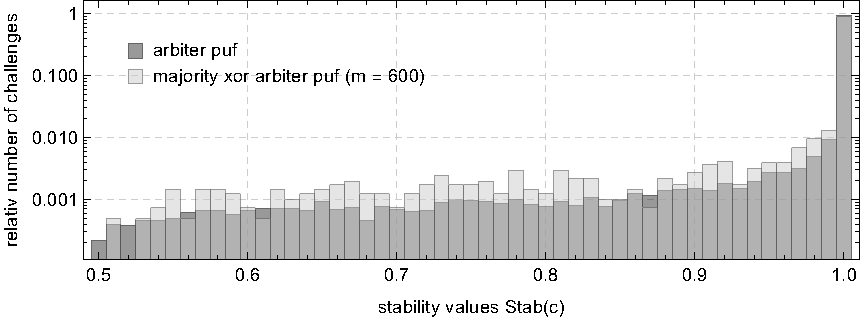
\includegraphics[width=1.00\textwidth]{images/comparison-arbiter-stability-distribution-majority-xor-stability-distribution_mono.pdf}  
    \fi
\fi
% \noindent\includegraphics[width=1.00\textwidth, height=3cm, draft]{example-image-a}
\caption[Challenge stability distribution of a Majority \acs{XOR} \apuf]{The histogram shows the relative frequency of the challenge stability values clustered into buckets of a \mxpuf with size $\gls{k} = 32$ and $32$ stages each in comparison to the challenge stability distribution of an \apuf, as shown in Fig.\ \ref{fig:arbiterstabilitydistribution}. \ac{MV} uses $\gls{m} = 600$ to reach a stability of $95\ \%$ with likelihood $95\ \%$ for randomly chosen challenges. The distribution and the amount of unstable challenges of the \mxpuf resembles the distribution of an \apuf.} 
\label{fig:comparisonarbiterstabilitydistributionmajorityxorstabilitydistribution}
\end{figure}

This shows that even large \mxpufs can become stable through a feasible number of votes and even exceed stability of a basic \apuf with a larger number of \ac{MV}.

%========================================
% fig:stabilitydistributionmajorityvote: direct comparison? it's hard to compare on different pages
% fig:stabilitydistributionmajorityvote: could the not-so-smooth histogram be caused by the effects of 'even number of errors cancel out'?











